%----------------------------------------------------------------------------------------
%	PACKAGES AND OTHER DOCUMENT CONFIGURATIONS
%----------------------------------------------------------------------------------------

\documentclass{article} % paper and 12pt font size
\usepackage{amsmath,amsfonts,amsthm} % Math packages
\usepackage[margin=1in]{geometry}
\usepackage{graphicx}
\usepackage{float}
\usepackage[parfill]{parskip}
\usepackage[labelsep=quad,indention=10pt]{subfig}
\setlength{\paperwidth}{8.5in}
\setlength{\paperheight}{11in}

%----------------------------------------------------------------------------------------
%	TITLE SECTION
%----------------------------------------------------------------------------------------

\newcommand{\horrule}[1]{\rule{\linewidth}{#1}} % Create horizontal rule command with 1 argument of height

\title{	
\normalfont \normalsize 
\textsc{University of Texas at Austin, CS 394N} \\
\horrule{0.6pt} \\[0.4cm] % Thin top horizontal rule
\huge Homework 4 - Game Agents \\[0.4cm]
\large Write Up  \\
\horrule{2pt} \\[0.5cm] % Thick bottom horizontal rule
}
\author{Venketaram Ramachandran} % Your name
\date{\normalsize\today} % Today's date or a custom date

\begin{document}

\maketitle % Print the title

%----------------
% Approach
%----------------
\section{Experimental Observations}
Before I proceeded to create a tournament team or maneuver walls, I wanted to observe vanilla agents and cowards. My goal was to use this information to better inform my intuition on what type of team to utilize.

\subsection{Vanilla Agents}
In order to get a baseline on the agents, I attempted to run the simulation without explicitly performing any training. I sought to answer the following questions: \textit{What does an agent do without any training? With what am I starting?} 
\\[1\baselineskip]
Without any sort of specification, the natural tendency of the agents seemed to be to randomly move and disperse. The behavior was largely expected given that there is randomness as the agents evolve and the fact that there wasn't any specific reward for any of the particular agent behavior. The vanilla agent setup is located in the file: vanilla-team.txt.

\subsection{Cowards}
I wanted to test the applicability of trying to stay alive as long as possible by fleeing immediate battle. As such, I wanted to test a batch of agents that fled an enounter as quick as they could. I labeled this batch of agents 'Cowards.' The only brief training performed on the Cowards was to have a parameter value of -100\% for "Approach Enemy" in the midst of several turrets. The trained team is located at: cowards.txt

In general, the Cowards team was pitted against the vanilla team and won handily (i.e. 148-24) when the battle was terminated. Though the vanilla team is not the best of benchmarks, the actions exhibited during the battle were intriguing. 

Specifically, the Cowards team was able to establish an agent count advantage by immediately picking off the agents that crossed the wall and wandered into the region that spawned the Cowards team. In addition, the Cowards simulated the behavior of standing ground after the Cowards went all the way to the walls at the environment boundaries. The Cowards team picked off opposing agents that came nearby due to a agent count advantage.

\section{Going Around the Wall}
For agents, going around the wall could potentially be a major issue and potentially inhibiting to their overall strategy. In order to tackle the problem of the wall, I decided to utilize the flag to help navigate around the main wall. 
\subsection{Initial Approach}
In my first attempt, I simply set the flag and the agent spawn locations on the exact opposite side of the main wall. I made the reward 100\% for approaching the flag. All other parameters were zero. I anticipated that some population of agents would evolve and go around the wall, especially given that there was a large reward.

\begin{figure}[H]
	\centering
		\subfloat{%
    		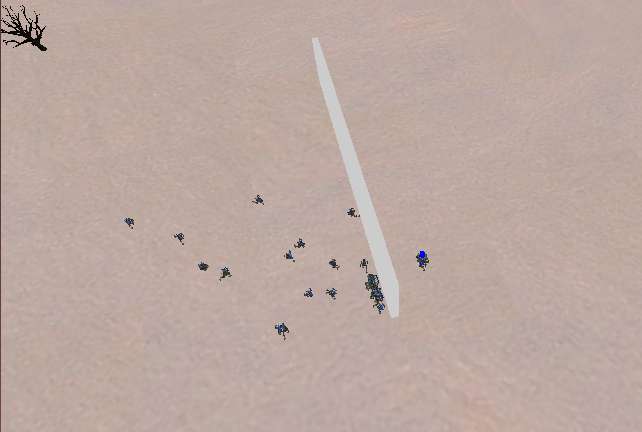
\includegraphics[height=5cm]{GoalFinding.png}%
            \label{fig:left}%
            } 
		\caption{\textit{Agents training to approach the goal.}}
        \label{fig:default}
\end{figure} 

\subsection{Insight and Improvement}
My initial approach mainly ended in me waiting for hours without the agents truly making much progress in getting to the other side of the wall. I reasoned that this was due to the fact that I was expecting some sort of randomized evolutionary change and having that evolve into a dominant population trait. In this case, the chance that such a complex behavior would randomly develop and propagate into a dominant population trait would be too difficult or take significant amounts of time. Instead, I approached the problem in steps.
\\[1\baselineskip]
First, I attempted to develop a population with a flag-seeking behavior as suggested in 4a) in the homework prompt. I allowed for the flag to be far enough away from the spawning point but the path to the flag was unobstructed. The following figure shows the initial step.

\begin{figure}[H]
	\centering
		\subfloat{%
    		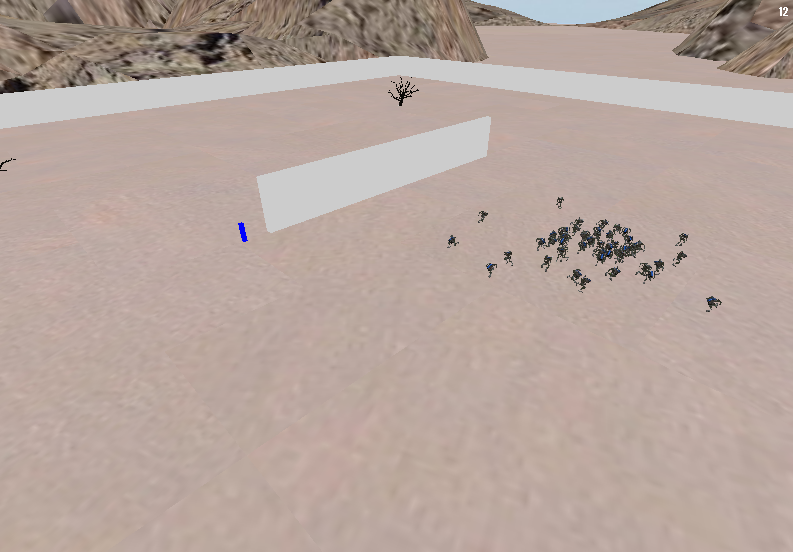
\includegraphics[height=5cm]{GoalFinding2.png}%
            \label{fig:left}%
            } 
		\caption{\textit{Agents training to approach the goal.}}
        \label{fig:default}
\end{figure} 

Once the agents were able to locate the goal, I gradually moved the goal further and further behind the wall. The final position was directly aligned with the center of the wall. The agents spawning was placed directly on the opposite side of the wall. Eventually, the agents were able to accurately go behind the wall. Figure 3 illustrates the overall gradual training process in an abbreviated fashion.

\begin{figure}[h]%
	\centering
    	\subfloat[Slightly obstructed by the wall]{%
        	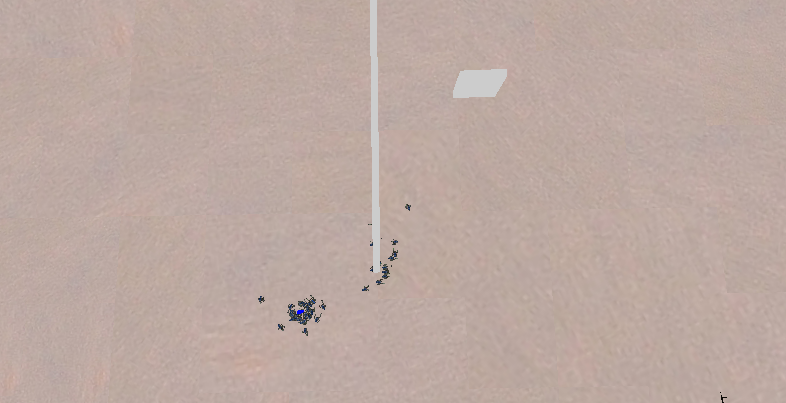
\includegraphics[width=50mm]{wallMasters.png}%
            \label{fig:left}%
        }\hfill%
        \subfloat[Slightly behind the wall]{%
        	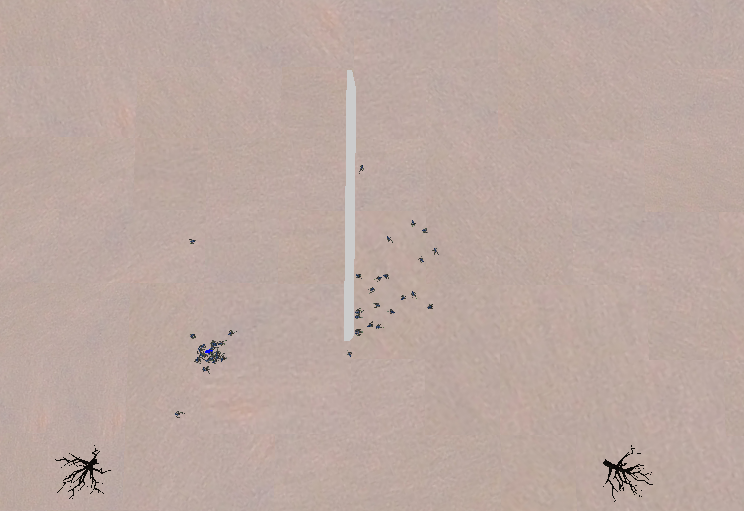
\includegraphics[width=50mm]{WallMasters2.png}%
            \label{fig:middle}%
        }\hfill%
        \subfloat[At the center of the wall]{%
        	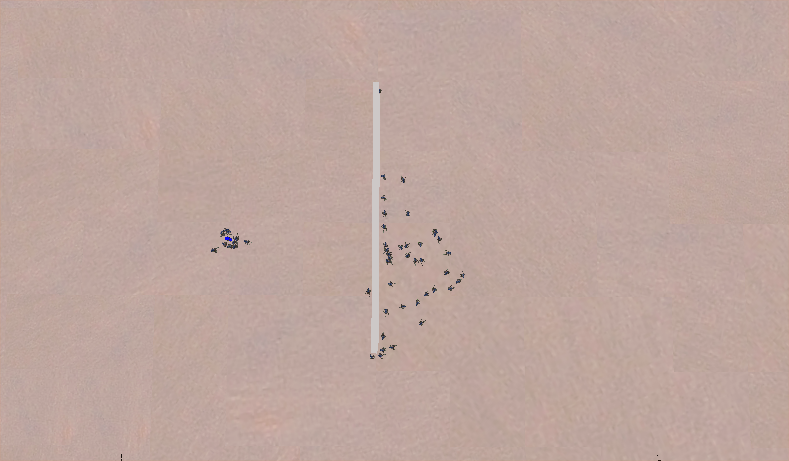
\includegraphics[width=50mm]{WallMasters4.png}%
            \label{fig:right}%
        }
    \caption{\textit{Agents learning to go around the wall for a goal.}}
    \label{fig:default}
\end{figure}  

\subsection{Parameters}

\begin{table}[H]
\centering
\begin{tabular}{l|r}
Reward Component & Quantity (in \%) \\\hline
Approach Flag & 100 \\
Stand Ground & -50
\end{tabular}
\caption{\label{tab:widgets}Parameter values used for wall maneuvering.}
\end{table}
As shown in Table 1, I mainly leveraged non-zero values for the following two parameters, listed in my perceived order of importance: "Approach Flag" and "Stand Ground." The following explains my rationale for the parameters I chose:

\begin{enumerate}
\item \textit{Approach Flag} - The most important task was to find the goal. As a result, I kept the weight of the "Approach Flag" value at a full 100\%.
\item \textit{Stand Ground} - I updated the "Stand Ground" value to have a negative weight of -50\%. From my initial failure of getting the agents around the wall, I noticed that the agents slamming their faces into the wall do not essentially move. I intuited that a reward for not standing in the same place would help the agents achieve their goal faster. I wanted to ensure that this value was a fair bit less than the reward for "Approach Flag" as I did not want the main goal of the agents to conflict between to "Approach Flag" and to not "Stand Ground."
\end{enumerate} 

Figure 3 shows the weight values towards the tail end of the training.

\begin{figure}[H]%
	\centering
    	\subfloat{%
        	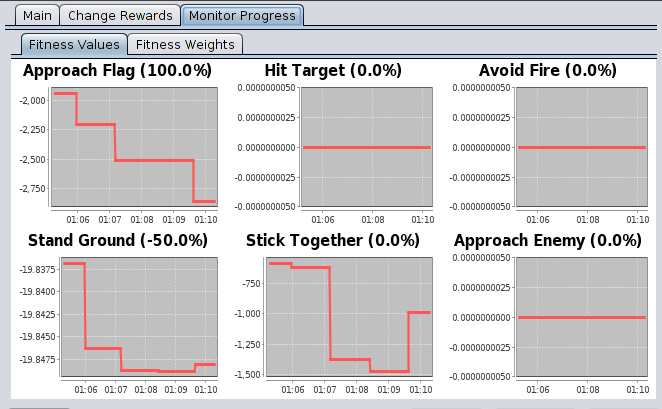
\includegraphics[height=5cm]{WallMasterValues.png}%
            \label{fig:left}%
        }\hfill%
    \caption{\textit{Weight values towards the end of wall manuevering training.}}
    \label{fig:default}
\end{figure} 

Given the difficulty, in both a time and complexity sense, of training the agents to navigate around a wall, I utilized the wall maneuvering as a starting point for the different agents that I trained.

\section{Submission Team Composition}
As mentioned in the previous section, the starting point for the team was the saved file for maneuvering around a wall.
\subsection{Motivation}
Based on the my experimentation with cowardliness behavior above, I decided to compose a 'cowardly' team. Though I realize that corwardice might not win against all possible teams, I concluded it might be an interesting approach to take. 
\\[1\baselineskip] In addition, from looking at the homework suggestions as well as communication I've had with my peers in the course, I anticipate aggressive teams. Given that both teams start from behind the wall, in order to engage one another, some subset of agents will first come out from behind the wall. With a cowardly approach, my team will not actively seek to engage and will instead wait for the agents from the opposing team to come out. Once opposing team members approach the area across the wall, the cowardly team could fire at them with a large unit, while navigating backwards. I hypothesized that the cowardly team may be able to create an agent count advantage as it did with the vanilla team above.
\subsection{Parameters}

\begin{table}[H]
  \centering
  \begin{tabular}{l|r}
  Reward Component & Quantity (in \%) \\\hline
  Approach Enemy & -100 \\
  Hit Target & 80 \\
  Stick Together & 30 \\
  Avoid Fire & 10 \\
  Approach Flag & 0 \\
  Stand Ground & 0 
  \end{tabular}
  \caption{\label{tab:widgets}\textit{Parameter values used for Cowardice-based team.}}
\end{table}

As shown in Table 2, I mainly leveraged non-zero values for the following four parameters, listed in my perceived order of importance: "Approach Enemy," "Hit Target," "Stick Together," and "Avoid Fire." The following explains my rationale for the parameters I chose:

\begin{enumerate}
\item \textit{Approach Enemy} - This was the most important task from my perspective. I wanted the agents to flee upon perceiving an enemy, in order to either prolong longevity or draw the enemy into an unfavorable situation in terms of agent numbers. As a result, I set this parameter at a full -100\%.
\item \textit{Hit Target} - In order for my strategy of cowardice to work, I required the "Hit Target" parameter to be quite high as well. I needed the agents to be able to fire at enemy as they retreat from an enemy or if the enemy was close. As a result, I set this parameter quite high, at 80\%, but still less than the "Approach Enemy" parameter.
\item \textit{Stick Together} - If the agents retreat but generally separate, then the chasing enemy can outnumber and overpower the separated agents. Therefore, I placed emphasis on "Stick(ing) Together," though, to me, being able to "Stick Together" was not as important as being able to "Hit Target" and to not "Approach Enemy."
\item \textit{Avoid Fire} - Avoiding fire might seem a bit counterintuitive. However, from a defensive and retreating perspective, I wanted to make sure that there was a nudge in order to not overly be selected by "Hit Target" and not to engage the enemy directly.
\end{enumerate}

The "Approach Flag" is useful in teaching the agents particular behavior such as going around a wall. Beyond going around walls, I've not needed for the "Approach Flag" for any teaching contexts. Similarly, the "Stand Ground" flag was not something I saw an intuitive need to use. In certain contexts, such as against the boundaries of the game world, the agents may not need a nonzero movement velocity. In other contexts, such as running away, the agent may need it. In general, I found that I did not have any behavior in mind for the agents that necessitated the use of the "Stay Ground" flag.

\subsection{Training Methodology}
In order to train the Cowards, I leveraged multiple turrets, generally upwards of six to eight turrets. 

I first trained the Cowards to be able to flee. I flanked the agent spawning point on each side with turrets. I set the -100\% value for "Approach Enemy" and 10\% value for "Avoid Fire" first and nothing else, with the intention that I wanted to develop the behavior to flee away from the enemy. Fairly soon, I saw that the agents began to develop behavior that suggested that they were trying to avoid the turrets. Specifically, the majority began to start straying away from the turrets or tried to move to locations that was out of turret line of fire. 
\\[1\baselineskip]
Once I saw this, I set my 30\% value for "Stick Together," wanting to make sure that agents somewhat moved together. Soon, the agents began displaying behavior of generally moving together, if the opportunity presented itself.
\\[1\baselineskip]
With these three parameters, the agents began to develop some interesting behaviors. For example, the agents moved in single file lines and hid behind walls, if necessary, to avoid the turrets. Similarly, if it was most safe to be clumped in an area away from the turrets, the agents exhibited that behavior. Figure 5 below depicts both behaviors.

\begin{figure}[H]%
	\centering
    	\subfloat[Single-file line to behind the wall]{%
        	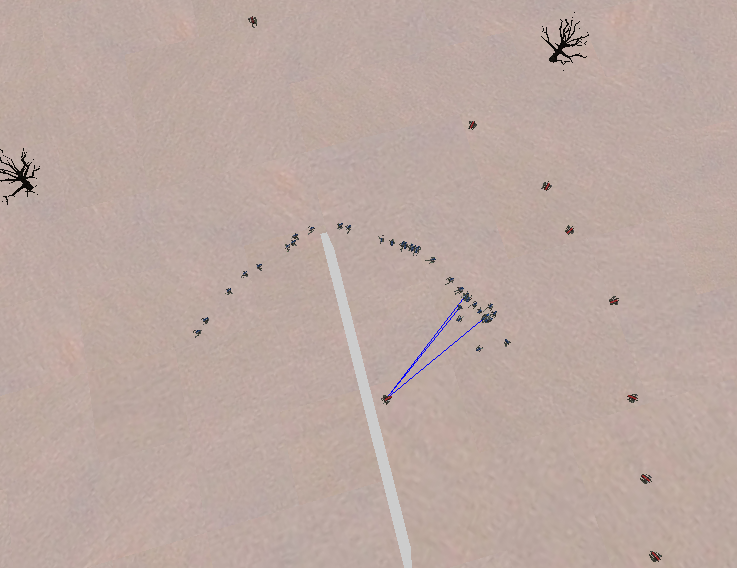
\includegraphics[height=5cm]{CowardsAroundWall.png}%
            \label{fig:left}%
        }\hfill%
		\subfloat[Safe positions away from the turrets]{%
        	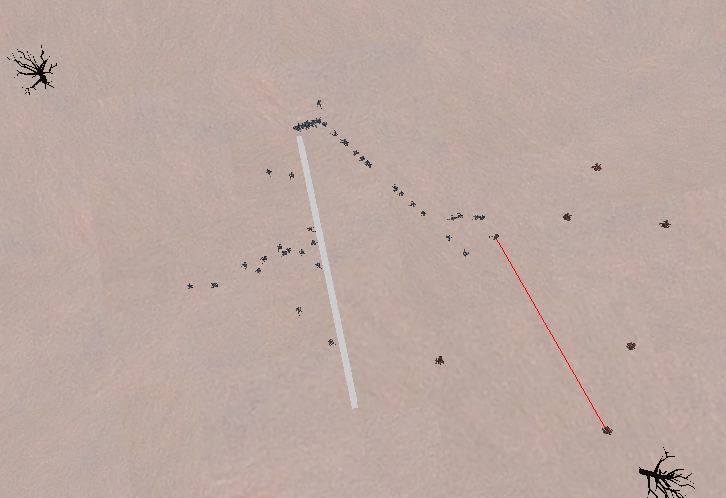
\includegraphics[height=5cm]{CowardsBehindWall.png}%
            \label{fig:right}%
        }\hfill%
    \caption{\textit{Behavior learned by the Coward team.}}
    \label{fig:default}
\end{figure} 

Finally, the parameter to "Hit Target" was increased to 80\%. However, to speed up the agent training a bit, I encircled the agent spawning location with turrets. Figure 6(a) depicts this setup. I reasoned that, eventually, the population that grows to fire at the turrets would become dominant. I also reasoned that this setup would not erase any of the previous traits that were learned by the agents and merely help along the process of getting the agents to consitently fire at the enemy as long as the process was not significantly long. As I had suspected, once the agents were let out of this scenario by removing two of the turrets, they immediately tried to get away from the remaining turrets but did so while firing at them. This behavior is depicted in figure 6(b).

\begin{figure}[H]%
	\centering
    	\subfloat[Encircled by turrets]{%
        	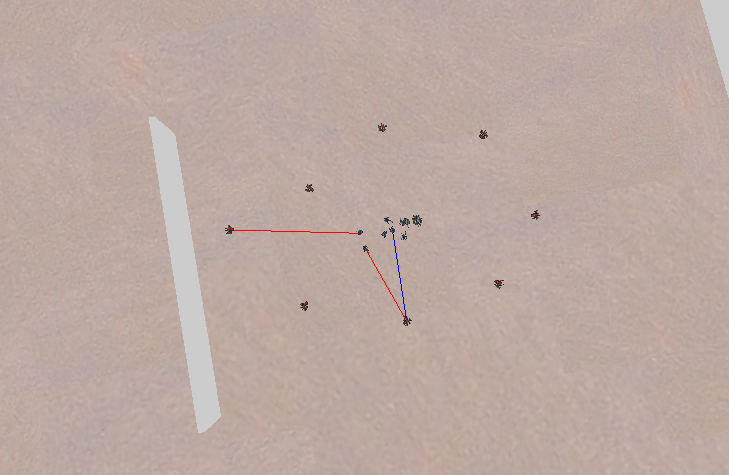
\includegraphics[height=5cm]{TurretCircle.png}%
            \label{fig:left}%
        }\hfill%
    	\subfloat[Escaping the circle of turrets]{%
        	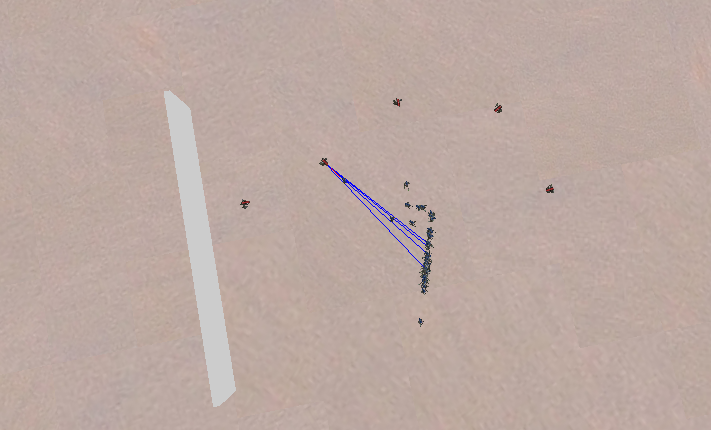
\includegraphics[height=5cm]{TurretEscape.png}%
            \label{fig:right}%
        }\hfill%
    \caption{\textit{Training the agents to fire at targets.}}
    \label{fig:default}
\end{figure} 

I, then, experimented by placing random turrets in locations to which the agents had escaped. As expected, the agents immediately began firing while escaping away from the turrets. After further tinkering with the agents (i.e. forcing them go around walls, adding extra walls, and adding more random turrets), I decided that the agents effectively exhibited the behavior that I wanted to see in them. 

\subsection{Testing the Team}

I tried my team against a simple, but relatively more aggressive team as specified in part 4 of the homework specifications. I created the aggressive team solely for the purpose of testing. Given that one of my initial goals for the coward team is to take advantage of aggresiveness, this was an appropriate opponent group to compare my agents. The following section  describes the parameters and training for the aggresive agents. The section after describes the results. Given that the focus of this document is not on the test agents, the descriptions are quite brief.

\subsubsection{Battle Opponent}

The aggressive team's base template came from the template trained to go around walls. The training followed the training regimen recommended in section 4 of the homework specifications almost identically. The following table describes the parameters used for training:

\begin{table}[H]
  \centering
  \begin{tabular}{l|r}
  Reward Component & Quantity (in \%) \\\hline
  Approach Enemy & 80 \\
  Hit Target & 100 \\
  Stick Together & 40 \\
  Avoid Fire & 0 \\
  Approach Flag & 0 \\
  Stand Ground & 0 
  \end{tabular}
  \caption{\label{tab:widgets}\textit{Parameter values used for the aggression-based team.}}
\end{table}

The following explains the rationale for the chosen parameters:

\begin{enumerate}
\item \textit{Hit Target} Given the aggression, the agent needed to be trained in mainly being able to ensure that the agent is able to hit the target. Otherwise, the agent loses its purpose. 
\item \textit{Approach Enemy} If the agent approaches the enemy, but doesn't fire, it also loses its purpose. Therefore, the approaching of the enemy is given a weight of 80\%, slightly less than "Hit Target."  
\item \textit{Stick Together} A larger group may be able to attack more efficiently. However, this is not as important as the other two parameters.   
\end{enumerate}

As mentioned in the specification for the homework assignment, the agent was first trained to approach enemies (i.e. increase the "Approach Enemy" parameter) and then to hit the enemy while approaching them (i.e. increase the "Hit Target" parameter). Lastly, the population was trained to stick together (i.e. increase the "Stick Together" parameter).

\subsubsection{Battle Results}

In battles, the Coward team won handily against the aggresive team. Generally, the battles never ended with all agents being eliminated. I terminated the battles after some time. Figure 7 depicts two of these results. 

\begin{figure}[H]%
	\centering
    	\subfloat[Battle 1: Coward team wins 376-208]{%
        	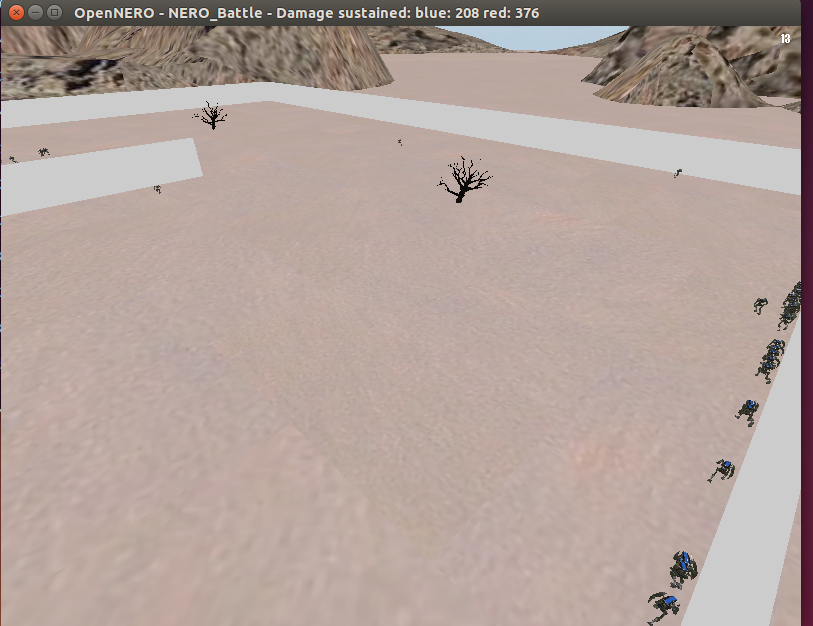
\includegraphics[height=5cm]{CowardBattle2.png}%
            \label{fig:left}%
        }\hfill%
    	\subfloat[Battle 1: Coward team wins 472-258]{%
        	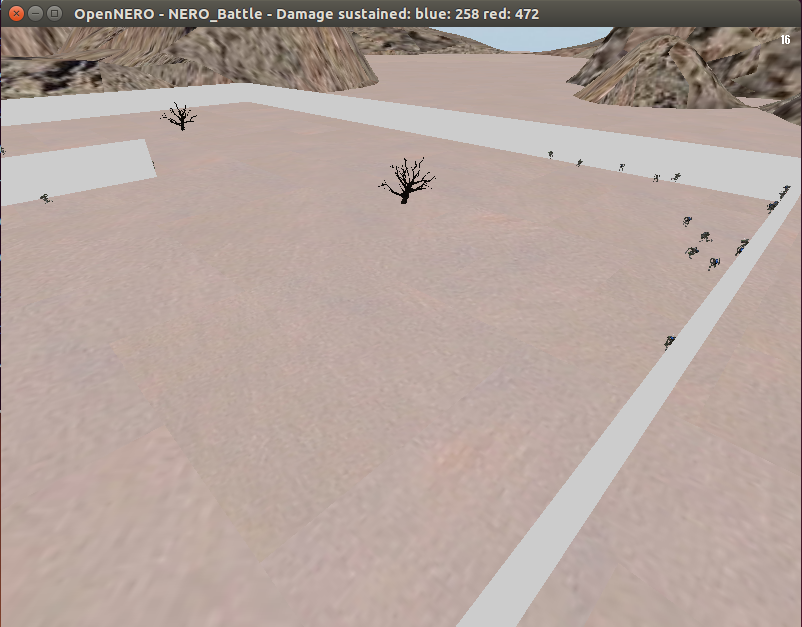
\includegraphics[height=5cm]{CowardBattle3.png}%
            \label{fig:right}%
        }\hfill%
    \caption{\textit{Two battles between the Coward team and the suggested team in the homework spec's section 4.}}
    \label{fig:default}
\end{figure} 

\subsubsection{Against Itself}
I tried to also run a battle against the Coward team itself. As expected, given the nature of the team's tendencies, the battle rarely had any action and any combat. I terminated the battle without a winner.
\\[1\baselineskip]
Given the results, I am currently satisfied with the constructed agent enough for submission. 

\section{Areas of Improvement for OpenNERO}
The following sections describe ways in which this experience can be made better.
\subsection{Bugs}
\begin{itemize}
\item When swapping from "Multi-Agent Battle Mode" to "Multi-Agent Training Mode" and back to "Multi-Agent Battle Mode," the dialog input box to load red and blue teams does not load. OpenNERO has to be terminated and started once again for the "Multi-Agent Battle Mode" to load.
\item After selecting the "Multi-Agent Training Mode," a dialog shows up to load a team, start a team, and control fitness values. However, there is a gap between the starting of the mode and the appearance of the dialog box. If the world view is panned or rotated before and as the dialog box shows up, the last action on the camera will continue forever (e.g. a pan left will continue left forever and out of bounds). The only resolution I found was to exit the program and restart it. 
\item When either pressing 'F' or 'C', after a certain threshold, the orientation of the camera abruptly changes or the camera is reset to a different position in the field.
\item If a turret is placed right on or near a tree, it becomes almost impossible to remove the turret. Right-clicks, at least in the numerous times I tried it at various poses and zoom, did not register the object to provide the option for removal.
\end{itemize}
\subsection{Suggestions}
\begin{itemize}
\item It was inconvenient that the training of the agents had to happen in real time. Often, this meant that the waiting time for certain group of population with particular behavior took a long period of time (i.e. in my case, it was on the order of hours). Any mechanism of speeding up the simulations might be useful. 
\end{itemize}
\end{document}